\section{Measuring parametrization effects}
\label{sec:parametrizing}

After implementing the \ac{pimc} search previously described, some tests were executed in order to observe the effects of different parametrizations.
However, these tests had to be comparative and a baseline was required to establish a standard measure.


\subsection{Rule-based Agent}
The baseline agent was called Rule-based and its main idea was to chose a move considering predefined rules, instead of using hard computational algorithms.
The following pseudo-code illustrates the deliberation process of this agent and tries to roughly reproduce the reasoning of a non-professional human player.

\begin{algorithm}
	\caption{Rule-based Sueca algorithm}
	\begin{algorithmic}[1]
		\Procedure{RuleBasedDecision}{InfoSet $I$}
			\State $HighestCardPerSuit$ = GetHighestCardPerSuitFromHand($I$)
			\ForAll {$h \in HighestCardPerSuit$}
				\If{isHighestUnplayedFromSuit($h$)}
					\If{GetSuit($h$) = TRUMP \&\& CountCardsFromSuit($I$) > 5}
						\State \textbf{return} h
					\ElsIf{GetSuit($h$) $\not=$ TRUMP \&\& CountCardsFromSuit($I$) > 5}
						\State \textbf{break}
					\ElsIf{GetSuit($h$) $\not=$ TRUMP}
						\State \textbf{return} h
					\EndIf
				\EndIf
			\EndFor
			\State \textbf{return} GetLowestCardFromHand($I$)
		\EndProcedure
	\end{algorithmic}
	\label{alg:pimc}
\end{algorithm}

It starts by collecting the highest cards of each allowed suit for the current play.
The possibility of playing such a highest card is granted by two requirements: being the highest unplayed card of that suit; and not holding at least other 5 cards from that suit, except for the trump suit.
Otherwise, this rule-based player return the lowest possible card.

The first experiments to test this baseline player compare three different scenarios:
\begin{itemize}
\item (a) 1000 games with 4 Rule-based players;
\item (b) 1000 games with 1 Rule-based player and 3 Random players;
\item (c) 1000 games with 2 Rule-based players against 2 Random players.
\end{itemize}

\begin{figure}[h]
        \centering
        \begin{subfigure}[h]{0.32\textwidth}
                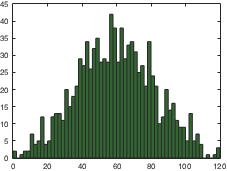
\includegraphics[width=\textwidth]{./img/5/HA-4RuleBased}
                \caption{Scenario A}
                \label{fig:histogramA}
        \end{subfigure}
        \begin{subfigure}[h]{0.32\textwidth}
                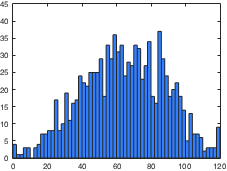
\includegraphics[width=\textwidth]{./img/5/HB-1RuleBased_3Random}
                \caption{Scenario B}
                \label{fig:histogramB}
        \end{subfigure}
        \begin{subfigure}[h]{0.32\textwidth}
                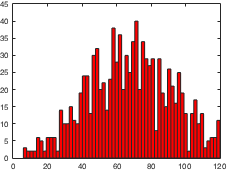
\includegraphics[width=\textwidth]{./img/5/HC-2RuleBased_2Random}
                \caption{Scenario C}
                \label{fig:histogramC}
        \end{subfigure}
        \caption[Histograms of the final points obtained in the 3 scenarios]{Histograms of the final points obtained in 1000 games by: (a) one of the teams; (b) the team with 1 Rule-based player and 1 Random player; (c) the team with 2 Rule-based players}
        \label{fig:histograms}
\end{figure}

In scenario A, results are very balanced, as expected, because all players have the same deliberation process.
In 1000 games one of the teams obtained a winning percentage of 48,5\% and a drawing percentage 1,9\%.
The scenario B shows that a team with 1 Rule-based player and 1 Random player can beat a 2 Random players team 56,6\% othe games





